%%%%%
%%Title: HiPi+Bus V0.2 Chapter 6
%%Creator: Ando Ki
%%CreationDate: April 1992
%%FileName: sec3
%%RelatedFile: ch6
%%%%%
\section{중재버스의 시간규격}
\subsection{ABRQ{\tt <}n{\tt >}*, DBRQ{\tt <}n{\tt >}*의 시간규격}
중재에 참가하기 위해서는 중재에 참가하고자 하는 버스클럭 주기에
해당 버스클럭의 백플레인의 하강점에서 $TP^{ARB}_1$ 시간 이후부터
$TP^{ARB}_0$ 동안 해당 중재요청신호를 백플레인에 안정되게 구동하여야 한다.
이때 중재요청신호의 전달지연시간은 $TP^{ARB}_2$로 규정한다.
중재 주기에서 중재를 수행한 결과 버스 사용권을 획득한 중재기는 자신의 중재요청신호의
구동을 이어지는 중재에 여향을 미치지 않도록 충분히 빨리 신호구동을 멈추어야 하고
이때 $TP^{ARB}_3$를 보장하여야 한다.
나머지 중재기들은 중재요청신호를 계속 구동하여 이어진 중재주기로 중재동작을 계속하게 된다.
%\documentstyle[a4]{hbook}
%\begin{document}
%
\begin{table}[htbp]
\caption{중재버스 신호의 시간규격 요약}\label{table:arb-time}
   \begin{center}
   \begin{tabular}{|l|l|r|r|r|} \hline
	timing parameter & name & min & typical & max \\ \hline \hline
	$TP^{BCLK}_0$ & BCLK* cycle time & 59 & 60 & 61 \\ \hline
	$TP^{ARB}_0$  & arbitration time & - & 50 & - \\ \hline
	$TP^{ARB}_1$  & pre-time & - & - & 10 \\ \hline
	$TP^{ARB}_2$  & bus propagation time & - & - & 20 \\ \hline
	$TP^{ARB}_3$  & off time & 10 & - & 15 \\ \hline \hline
	$TP^{INH}_0$  & ABINH time & 25 & 30 & 35 \\ \hline
	$TP^{INH}_1$  & bus propagation time & - & - & 20 \\ \hline
	$TP^{INH}_2$  & off time & 10 & - & 15 \\ \hline
   \end{tabular}
   \end{center}
\end{table}
%
%\end{document}

\begin{figure}[htb]
    \centerline{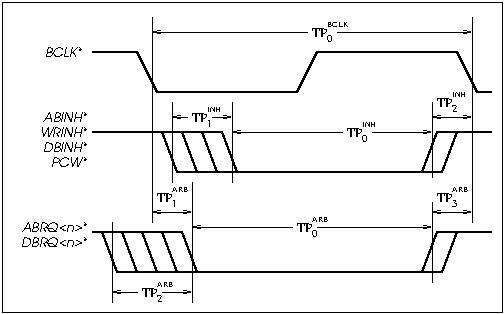
\includegraphics{ch6/FIG/arb-time.jpg}}
   \caption{중재버스의 시간규격}\label{figure:arb-time}
\end{figure}
%
\subsection{ABINH*, WRINH*, DBINH*의 시간규격}
이 신호는 중재요청신호의 구동을 제한하는데 사용하며
$TP^{INH}_0$ 시간동안 안정된 신호로 유지되어야 한다.
연속해서 여러 버스 사이클 동안 구동하는 경우, $TP^{INH}_1$ 시간은 무시하고
처음 구동 사이클에서 지킨다.
연속해서 여러 버스 사이클 동안 구동하는 경우, $TP^{INH}_2$ 시간은 무시하고
마지막 구동 사이클에서 지킨다.
%
%%%%%
